\subsubsection{\stid{3.12} Sub-project: hypre}

\paragraph{Overview}
The {\sl hypre} software library \cite{hypre:homepage,hypre_design_impl_2006} provides high performance preconditioners and solvers for the solution of large sparse linear systems on massively parallel computers, with particular focus on algebraic multigrid solvers. One of {\sl hypre}’s unique features is the provision of a (semi)-structured interface, in addition to a traditional linear-algebra based interface. The semi-structured interface is appropriate for applications whose grids are mostly structured, but with some unstructured features. Examples include block-structured grids, composite grids in structured adaptive mesh refinement (AMR) applications, and overset grids. These interfaces give application users a more natural means for describing their linear systems, and provide access to methods such as structured multigrid solvers, which can take advantage of the additional information beyond just the matrix. Since current architecture trends are favoring regular compute patterns to achieve high performance, the ability to express structure has become much more important. The {\sl hypre} library provides both unstructured and structured multigrid solvers, which have shown excellent scalability on a variety of high performance computers, e.g Blue Gene systems (unstructured solver BoomerAMG has scaled up to 1.25 million MPI cores with a total of 4.5 million hardware threads). It is used by many ECP application teams, including ExaAM, Subsurface, ExaWind, CEED, and more. It requires a C compiler and an MPI implementation, but it also runs in an OpenMP environment. It also has GPU capabilities.

\paragraph{Key  Challenges}

While {\sl hypre}'s solvers contain much parallelism, their main focus is the solution of sparse linear systems, leading to  very large demands on memory bandwidth. In addition, the use of multiple levels, while greatly aiding convergence of the solvers, leads to decreasing systems sizes, number of operations and parallel efficiencies on coarser levels. Particularly the unstructured algebraic multigrid solver BoomerAMG\cite{HeYa2002}, which is {\sl hypre}'s most often used preconditioner, suffers from increasing communication complexities on coarser levels. Coarse grid operators are generated by multiplying three matrices leading to increasing numbers of nonzeroes per row in the resulting matrices and with it increasing numbers of neighbor processes. While BoomerAMG's solve phase mainly consists of matrix vector products and smoothing operations, which are fairly straight forward to parallelize, even on a GPU, its setup phase is highly complex, including many branches, a lot of integer operations as well as some sequential passages. Previous interpolation strategies that lead to best convergence and performance on distributed memory machines were not suitable for implementation on GPUs or similar architectures requiring extreme parallelism and required new algorithmic approaches. Since {\sl hypre} is a mature product with many solvers and interdependent features, any significant changes that affect the whole library, are tedious and require much testing to ensure that the library stays backward compatible and no features are broken.

\paragraph{Solution Strategy}

Since computer architectures continue to change rapidly, it was important to come up with strategies that will facilitate future porting of the software. Therefore we developed and implemented a new memory model that addresses the use of different memory locations.
Since the upcoming computer architectures are heterogeneous with accelerators, we focus on enabling {\sl hypre} for GPUs. We have looked into various options, such as the use of CUDA, OpenMP 4.5, as well as RAJA and Kokkos. We limited the latter three options to the structured interface and solvers which are more natural candidates for such an approach due to their use of macros, called BoxLoops, for loops. We adopted a modular approach for the unstructured interface, which relies on the restructuring the solver components to use smaller kernels that are and/or will be implemented in CUDA for Nvidia GPUs. Since hip is similar to CUDA, porting to AMD GPUs has been fairly straight forward. We are now investigating the use of a vendor conversion tool from CUDA to SYCL to port structured and unstructured solvers to upcoming exascale computers with Intel GPUs.

\paragraph{Recent Progress}

Previously we had enabled the structured interface and solvers, SMG and PFMG\cite{AsFa1996}, to completely run on GPUs, using CUDA, OpenMP4.5, RAJA and Kokkos, and have now also added hip to enable use on AMD GPUs.
For our unstructured AMG solver BoomerAMG, we had implemented suitable CUDA kernels for setup and solve phase, designed a new class of interpolation operators based on sparse matrix operations\cite{LiSY2020}, implemented it on GPUs and ported aggressive coarsening to the GPU. Recently, we added Umpire support for memory pooling on GPUs, which can significantly improve performance. We have enabled hypre's specialized solvers, including linear and eigensolvers for Maxwell problems and solvers for H-div problems, to run on Nvidia GPUs. Figure \ref{fig:AMS-PCG} shows some results for a Maxwell problem using finite elements of increasing order on 1 node of Lassen. We have ported many of the CUDA kernels and routines in the unstructured interface to hip to enable their use on AMD GPUs. We have also developed a new version of multipass interpolation based on matrix-matrix multiplications and implemented it in CUDA and hip. Multipass interpolation is a popular low-memory prolongation used with aggressive coarsening. Figure \ref{fig:Spock-AMG} shows a comparison of CPU and GPU runtimes on 2 nodes of Spock for a 3D diffusion problem with a 27-point stencil on a $n \times n \times n$ grid using AMG-PCG with aggressive coarsening on the first level for increasing $n$.

\begin{figure}[bth]
\centering
	\includegraphics[width=3.9in]{projects/2.3.3-MathLibs/2.3.3.12-SUNDIALS-hypre/AMS-PCG.png}
	%\includegraphics[width=3in]{AMS-PCG.png}
	\caption{\label{fig:AMS-PCG} Solution of a simple 3D electromagnetic diffusion problem corresponding to the 2nd order definite Maxwell equation  $\nabla \times \nabla \times E + E = f$ using AMS-PCG on 1 node of Lassen (4 GPUs vs. 40 CPU cores) using finite elements of increasing order on a Fichera mesh.}

\end{figure}

\begin{figure}[bth]
\centering
	\includegraphics[width=3in]{projects/2.3.3-MathLibs/2.3.3.12-SUNDIALS-hypre/spock-AMG-PCG.png}
	%\includegraphics[width=3in]{spock-AMG-PCG.png}
	\caption{\label{fig:Spock-AMG} Total times (setup plus solve times) on 2 nodes of Spock using AMG-PCG with aggressive coarsening and multi-pass interpolation for a 3D diffusion problem with a 27-point stencil on a $n \times n \times n$ grid. The CPU runs were performed with 8 MPI tasks with 16 OpenMP threads per MPI task, the GPU runs were performed on 8 AMD MI100 GPUs.}

\end{figure}

\begin{figure}[bth]
\centering
	\includegraphics[width=5in]{projects/2.3.3-MathLibs/2.3.3.12-SUNDIALS-hypre/crusher-AMG-PCG.png}
	%\includegraphics[width=5in]{crusher-AMG-PCG.png}
	\caption{\label{fig:crusher-AMG} Setup, solve times and Speedups of GPU over CPU performance on 1 node of Crusher using AMG-PCG with three different settings for a 3D diffusion problem with a 27-point stencil on a $n \times n \times n$ grid. The CPU runs were performed with 64 MPI tasks, the GPU runs were performed on 8 AMD MI250 GPUs. Solid lines use the GPU default settings, whereas dashed and dotted lines use in addition one level of aggressive coarsening with two-stage and multipass interpolation, respectively.}

\end{figure}

\paragraph{Early Access System Experiences}

We have tested {\sl hypre} performance on both Spock, see Figure \ref{fig:Spock-AMG}, and Crusher.  Figure \ref{fig:crusher-AMG} 
shows the Setup and Solve times for three different settings of AMG for increasing $n$ of a 3D diffusion problem on a $n \times n \times n$ grid. Both CPU and GPU runs use the same settings. Solid lines use the default AMG settings, whereas dashed and dotted lines use one level of aggressive coarsening with two-stage and multipass interpolation, respectively. While generally systems in application problems would be in the range of up to $n=300$, we here continue to increase the problem size until the GPU runs reach the memory limit to demonstrate memory usage for these different AMG settings. This is reached first for the default version, which requires a lot of memory, but also achieves the lowest number of iterations, followed by the use of aggressive coarsening with two-stage interpolation. The use of one level of aggressive coarsening combined with multipass interpolation allows solving the largest system illustrated using GPUs, since it has lower memory requirements at the cost of having the worst convergence.  

{\sl Hypre} release v2.24.0 contains support for Intel GPUs for the structured interface and solvers via SYCL and Kokkos and for the solve phase of unstructured solvers via SYCL. All these features have been tested on Arcticus.

\paragraph{Next Steps}

We will pursue the following tasks:

\begin{itemize}
\item We will continue to add new GPU capabilities to {\sl hypre} and improve the performance of current capabilities. We will thoroughly investigate the performance on AMD GPUs and begin porting to Intel GPUs.
\item We will test and evaluate performance of important hypre solvers on AMD and Intel GPUs, improve their performance and port additional components if necessary.
\end{itemize}
In addition, we will work with ECP application teams who are using {\sl hypre}, such as ExaWind, ExaAM, AMReX,  to achieve best performance by tuning the solvers for them and potentially implementing suitable algorithmic changes.
